\newpage
\section{Systems of Ordinary Differential Equations}
\subsection{}
Systems of ordinary differential equations have 1 dependent variable and 1 independent variable. Let's look at an example.

\begin{eg}
  Here is a system of 3 first order ordinary differential equations of dimension 3 
  \begin{align*}
    x'&=4x-7y+z^2\\
    y'&=2t-e^{t}y-z\\
    z'&=z^2+y^2-yx
  .\end{align*}
\end{eg}

We can also turn higher order ODE's into systems of first-order ODEs.
\begin{eg}
  Consider the equation $x''+7x''+7tx'+6x=t^2$. If we let $y=x',z=x''=y',x'''=z'$, then using the ODE,
  \[
  z'=t^2-6x+7ty-7z
  ,\]
  we can make a system of nonlinear, nonautonomous, nonhomogeneous ordinary differential equations.\footnote{After this system we went to chapter 2.6}
  \begin{align*}
    x'&=y\\
    y'&=z\\
    z'&=t^2-6x+ty-7z
  .\end{align*}
\subsection{Matrix Algebra}
A matrix is a rectangular array of numbers. 
\begin{eg}
  Consider $A=\begin{pmatrix} 2&3&1\\4&5&0 \end{pmatrix} $. $A$ has 2 rows and 3 columns, so its size is $2\times 3$. The $a_{ij}$ is an entry in $A$'s $i^{th}$ row and $j^{th}$ column.
\end{eg}
\begin{eg}
  Consider $B=\begin{pmatrix} 5&0&0\\0&-1&0\\0&0&3 \end{pmatrix} $, which is a $3\times 3$ matrix. This is also a square matrix, due to the size. $B$ is also a diagonal matrix, because it's only nonzero entries are on the main diagonals.
\end{eg}
An upper triangular matrix looks like 
\[
  \begin{pmatrix} 5&2&0\\0&-1&3\\0&0&3 \end{pmatrix} 
.\] 
A lower triangular matrix looks like
\[
  \begin{pmatrix} 5&0&0\\ \pi&-1&0\\-1&-\frac{1}{2}&3 \end{pmatrix} 
.\] 
\end{eg}
We can add and subtract matrices element-wise, but only if the matrices have the same size. We can also multiply a matrix by a scalar
\[
  3\begin{pmatrix} 4&5\\6&7 \end{pmatrix} =\begin{pmatrix} 12&15\\18&21 \end{pmatrix} 
.\] 
A row vector is $\begin{pmatrix} 2&3&1 \end{pmatrix} $, in this case the size would be $1\times 3$. A column vector looks like $\begin{pmatrix} 2\\3\\1 \end{pmatrix} $ with the size $3\times 1$. The zero vector is of size $n\times n$, and has $0$ in every index in the matrix. The transpose of a matrix reverses all of the columns and rows. Consider
\[
  \begin{pmatrix} 2&3&1\\4&5&6 \end{pmatrix} ^{T}=\begin{pmatrix} 2&4\\3&5\\1&6 \end{pmatrix} 
.\] 
Here are the properties of a transpose:
\begin{itemize}
  \item $\left( A^{T} \right)^{T}=A $
  \item $\left( A+B \right) ^{T}=A^{T}+B^{T}$
  \item $(kA)^{T}=kA^{T}$
  \item $\left( AB \right) ^{T}=B^{T}A^{T}$
\end{itemize}
Now we are going to start talking about matrix multiplication. Matrix multiplication is like the dot product. The $(i,j)^{th}$ entry of $AB$ is the dot product of the $i^{th}$ row of $A$ w/ $j^{th}$ column of $B$. Consider the following
\[
  \begin{pmatrix} 1&2&3 \end{pmatrix} \begin{pmatrix} 4\\5\\6 \end{pmatrix} =(1\times 4)+(2\times 5)+(3\times 6)= 32
.\] 
In order to do matrix multiplication, rows of $A$ must match the columns of $B$ and vice versa. Matrix multiplication is not commutative. 
\begin{eg}
  If we let $A=\begin{pmatrix} 1&4\\5&10\\8&12 \end{pmatrix}$ and $B=\begin{pmatrix} -4&7&-3\\1&-3&2 \end{pmatrix} $. Does $AB=BA$? This is not true, because matrices are equal if and only if all entries are equal. If we just multiply $BA$, we get \[
  \begin{pmatrix} -4&7&-3\\1&-3&2 \end{pmatrix}\begin{pmatrix} 1&4\\5&10\\7&12 \end{pmatrix}  = \begin{pmatrix}2&8\\2&-2\end{pmatrix} 
  .\] 
\end{eg}
Here are some properties of matrices. 
\begin{note}
  We must maintain the order from left to right.
\end{note}
\begin{itemize}
  \item $A(B+C)=AB+BC$
  \item $(A+B)C=AC+BC$
  \item $k(AB)=(kA)B=A(kB)$
  \item $ABC=(AB)C=A(BC)$
\end{itemize}
The identity matrix is a square diagonal matrix with ones on the diagonal. For example, the identity matrix of dimension 3 and 4 are the following 
\begin{align*}
  I_3&=\begin{pmatrix} 1&0&0\\0&1&0\\0&0&1 \end{pmatrix} \\
  I_4&=\begin{pmatrix} 1&0&0&0\\0&1&0&0\\0&0&1&0\\0&0&0&1 \end{pmatrix} 
.\end{align*}
With the identity matrix, if we multiply any matrix by the identity matrix, then we get the same answer. Back in lesson 2, we were given the general solution to a Cauchy-Euler ordinary differential equation as \[
  x(t)=C_1(1)+C_2t^3+C_3 \frac{1}{t^2}
.\] Let's find a particular solution satisfying $x(1)=2,x'(1)=4,x'(1)=0$. We can do this by taking the derivative and second derivative of our functions to get 
\begin{align*}
  x'(t)=3C_2t^2-2C_3t ^{-3}\\
  x''(t)=6C_2t+6C_3t ^{-4}
.\end{align*}
Now using our initial conditions
\begin{align*}
  x(1)=C_1+C_2+C_3=2\\
  x'(1)=3C_2-2C_3=4\\
  x''(1)=6C_2+6C_3=0
.\end{align*}
We can rewrite this in matrix form as \[
  \begin{pmatrix} 1&1&1\\0&3&-2\\0&6&6 \end{pmatrix} \begin{pmatrix} C_1\\C_2\\C_3 \end{pmatrix} =\begin{pmatrix} 2\\4\\0 \end{pmatrix} 
.\] We will call the first matrix, $A$, the second matrix, $\vec{x}$, and the third matrix, $\vec{b}$, so we must solve $A\vec{x}=\vec{b}$ for $\vec{x}$. We can solve this by doing the following techniques
\begin{enumerate}
  \item Cramer's Rule (See book appendix)
  \item Gaussian elimination
  \item (Left)-multiply by $A^{-1}$
  \item MATLAB: rref or $A / B$
\end{enumerate}

\begin{theorem}
  This is the invertible matrix theorem. If $A$ is square, either all of case 1 or all of case 2 statements are true. Either $A$ is non-singular [good] or $A$ is singular [bad]. \newline Considering case 1
  \begin{itemize}
    \item $det(A)\neq 0$
    \item $A\vec{x}=\vec{b}$ has exactly one solution $\vec{x}$ for each $\vec{b}$.
    \item $A\vec{x}=\vec{0}$ has only the trivial solution, $\vec{x}=\vec{0}$.
    \item The rows (and columns) are linearly independent.
    \item $A^{-1}$ exists.
  \end{itemize}
  Considering Case 2
  \begin{itemize}
    \item $det(A)=0$
    \item $A\vec{x}=\vec{b}$ has zero or infinite solutions
    \item $A\vec{x}=\vec{0}$ has infinite solutions.
    \item The rows (and columns) are linearly dependent.
    \item $A^{-1}$ does not exist.
  \end{itemize}
\end{theorem}
$A^{-1}$ is a square matrix such that \[
A^{-1}A=A A^{-1}=I
.\] We find $A^{-1}$ through the following methods
\begin{enumerate}
  \item $rref(A|I)\to(I|A^{-1})$
  \item $A^{-1}=\frac{1}{det(A)}\cdot adj(A)$ where $adj(A)$ is the transpose of the cofactor matrix.
\end{enumerate}
How do we use $A^{-1}$? Given $A\vec{x}=\vec{b}$, we must solve for $x$. In order to do this, we left multiply by $A^{-1}$ to get 
\begin{align*}
  A^{-1}A\vec{x}&=A^{-1}\vec{b}\\
  I\vec{x}&=A^{-1}\vec{b}\\
  \vec{x}=A^{-1}\vec{b}
.\end{align*}
If given a general $2\times 2$ matrix, $A=\begin{pmatrix} a&b\\c&d \end{pmatrix} $, we can find the inverse by doing 
\begin{align*}
  A^{-1}&=\frac{1}{ad-bc}\begin{pmatrix} d&-c\\-b&a \end{pmatrix} ^{T}\\
        &=\frac{1}{ad-bc}\begin{pmatrix} d&-b\\-c&a \end{pmatrix} 
.\end{align*}
The trace of $A$ ($trace(A)$) is the sum along the diagonal.
\newline
Let's write a linear system of first order differential equations in matrix form. If the equation is not first order, use Sect (4.1) technique to turn into 1st order system.
\begin{eg}
  Consider the following system 
  \begin{align*}
    x'&=x-y+z\\
    y'&=4x+y-5z+7\\
    z'&=7x-8y-9z
  .\end{align*}
  The $+7$ in the second equation makes this a nonhomogeneous ordinary differential equation with constant coefficients. We can rewrite this as $\vec{x}'(t)=A(t)\vec{x}+\vec{b}(t)$, where $\vec{x}(t)=$ a vector of dependent variables. In order to do this, let $\vec{x}(t)=\begin{bmatrix} x(t)\\y(t)\\z(t) \end{bmatrix} $. Using the equation from before, we can set \[
  \begin{bmatrix} x'\\y'\\z'\\ \end{bmatrix} =\begin{bmatrix} 1&-1&1\\4&1&-5\\7&-8&-9 \end{bmatrix} +\begin{bmatrix} 0\\7\\0 \end{bmatrix} 
.\] We can notice that all of our nonhomogeneous terms get moved into the $\vec{b}(t)$ matrix.
\begin{note}
  We might have $\begin{bmatrix} c \end{bmatrix} \vec{x}'=A\vec{x}+\vec{b}$. From here we would need to do the following 
  \begin{align*}
    c^{-1}c\vec{x}'=c^{-1}(A\vec{x}+\vec{b})\\
    \vec{x}'=c^{-1}A\vec{x}+c^{-1}\vec{b}
  .\end{align*}
\end{note}
\end{eg}
\begin{eg}
  Consider the following ordinary differential equation and put it into matrix form.
  \begin{align*}
    x''+4x'-4x+4y&=0\\
    y''-4y'+5y-2x'+3x&=\sin(t)
  .\end{align*}
  In order to solve this we need to let $u=x'$, which makes $u'=x''$, and we need to let $v=y'$, which lets $u'=-4x'+4x-4y$ and $v'=y''=4y'-5y+2u-3x+\sin(t)$. This makes our system 
  \begin{align*}
    u'&=-4u+4x-4y\\
    v'&=4v-5y+2u-3x+\sin(t)\\
    x'&=u\\
    y'&=v
  .\end{align*}
  Now we can turn this into our $\vec{x'}=A\vec{x}+\vec{b}$. This makes our equation \[
    \begin{bmatrix} u'\\v'\\x'\\y'\\ \end{bmatrix} =\begin{bmatrix} -4&0&4&-4\\2&4&-3&-5\\1&0&0&0\\0&1&0&0 \end{bmatrix} +\begin{bmatrix} 0\\ \sin(t)\\0\\0 \end{bmatrix} 
  .\] 
\end{eg}

\subsection{Eigenvalues and Eigenvectors of Square Matrices}
We are going to be using $\lambda$ for the eigenvalues and $\vec{v}$ for the eigenvectors.
\begin{definition}
  $\lambda$ and $\vec{v}$ are an eigenvalue/eigenvector of $A$ if \[
  A\vec{v}=\lambda\vec{v}, v\neq 0
  .\] 
\end{definition}

Our steps to find the eigenvector are the following:
\begin{enumerate}
  \item Find $\lambda$'s with $det(A-\lambda I)=0$ (polynomial in $\lambda$).
  \item For each $\lambda$ find its eigenvector $\vec{v}$ using $A\vec{v}=\lambda\vec{v}$ or $(A-\lambda I)\vec{v}=0$
\end{enumerate}
We need to make sure that $\vec{v}$ is a non-zero solution to the equation. This means that we will have infinite solutions because every multiple of an eigenvector is also an eigenvector.
\begin{eg}
  For $A=\begin{bmatrix} 4&2\\5&1 \end{bmatrix}$, find eigenvalues and eigenvectors. In order to find the eigen vector we take the deteminant of $A-\lambda I$ and set it equal to zero.
  \begin{align*}
    det(\begin{bmatrix} 4&2\\5&1 \end{bmatrix} -\lambda\begin{bmatrix} 1&0\\0&1 \end{bmatrix} )&=0\\
    \left| \begin{matrix} 4-\lambda&2\\5&1-\lambda \end{matrix} \right| &=0\\
    (4-\lambda)(1-\lambda)-10&=0\\
    4-5\lambda+\lambda^2-10&=0\\
    \lambda^2-5\lambda-6&=0\\
    \lambda&=6,-1
  .\end{align*}
  Now we need to solve for the eigenvectors. First, let $\lambda=6$. Let $\vec{v}=\begin{bmatrix} v_1\\v_2 \end{bmatrix}$.
  \begin{align*}
    \begin{bmatrix} 4-6&2\\5&1-6 \end{bmatrix} \begin{bmatrix} v_1\\v_2 \end{bmatrix} &=\begin{bmatrix} 0\\0 \end{bmatrix} \\
    \begin{bmatrix} -2&2\\5&-5 \end{bmatrix} \begin{bmatrix} v_1\\v_2 \end{bmatrix} =\begin{bmatrix} 0\\0 \end{bmatrix} 
  .\end{align*}
  If we put this back into equation form we get 
  \begin{align*}
    -2v_1+2v_2&=0\\
    5v_1-5v_2&=0\\
    \to v_1=v_2
  .\end{align*}
  So this means that $v_2\begin{bmatrix} 1\\1 \end{bmatrix} $ is an eigenvalue for $\lambda=6$ for all $v_2\neq 0$. Let's now solve for $\lambda=1:$
  \begin{align*}
    \begin{bmatrix} 5&2\\5&2 \end{bmatrix} \begin{bmatrix} v_1\\v_2 \end{bmatrix} &=\begin{bmatrix} 0\\0 \end{bmatrix} \\
    5v_1-1v_2=0\to v_2=\frac{-5}{2}v_1
  .\end{align*}
  This means that any multiple of the vector $\begin{bmatrix} 1\\-\frac{5}{2} \end{bmatrix}$ is an eigenvector for $\lambda=1$.
\end{eg}

Let's show that if $\vec{v}$ is an eigenvector for $A$ with $\lambda$, then $c\vec{v}$ is an eigenvector for $A$ with $\lambda$ if $c\neq 0.$. We know that $A\vec{v}=\lambda\vec{v}$. Is $A(c\vec{v})=\lambda(c\vec{v})$? Yes.
Let $X(t)=\begin{bmatrix} x(t)\\y(t) \end{bmatrix} $. If we solve for $\vec{X}'=A\vec{x}$, 
\begin{align*}
  \begin{bmatrix} x\\y \end{bmatrix} '=\begin{bmatrix} 4&2\\5&1 \end{bmatrix} \begin{bmatrix} x\\y \end{bmatrix} \\
  x'=4x+2y\\
  y'=5x+y
.\end{align*}
We can now write down our solutions as 
\begin{align*}
  \vec{X}_1(t)=e^{6t}\begin{bmatrix} 1\\1 \end{bmatrix} =\begin{bmatrix} e^{6t}\\e^{6t} \end{bmatrix} \\
  \vec{X}_2(t)=e^{-t}\begin{bmatrix} -2\\5 \end{bmatrix} =\begin{bmatrix} -2e^{-t}\\5e^{-t} \end{bmatrix} 
.\end{align*}
This means that we can determine that \[
  \vec{X}(t)=c_1\vec{x}_1+c_2\vec{x}_2
\] is also a solution for all $c_1,c_2$. This means that our general solution is going to be \[
\vec{X}=c_1e^{6t}\begin{bmatrix} 1\\1 \end{bmatrix} +c_2e^{-t}\begin{bmatrix} -2\\5 \end{bmatrix} 
.\] We can also take our $c_1,c_2$ and distribute them to get \[
\vec{X}(t)=\begin{bmatrix} c_1e^{6t}-2c_2e^{-2}\\c_2e^{6t}+5c_2e^{-t} \end{bmatrix} 
,\] with $x(t)$ being the top equation and $y(t)$ being the bottom equation. We can verify the solutions in order to convince ourselves that this works. We can verify by using our $\begin{bmatrix} -2e^{-t}\\5e^{-t} \end{bmatrix} $. Our left hand side of the equation is going to be \[
\vec{X}_2'=-e^{-t}\begin{bmatrix} -2\\5 \end{bmatrix} =e^{t}\begin{bmatrix} 2\\-5 \end{bmatrix} 
.\] Our right hand side of the original equation is going to be \[
A\vec{X}_2 = \begin{bmatrix} 4&2\\5&1 \end{bmatrix} e^{t}\begin{bmatrix} -2\\5 \end{bmatrix} 
.\] After simplification of this equation, we get that the result is $e^{t}\begin{bmatrix} 2\\-5 \end{bmatrix} $.
\begin{eg}
  Find the particular solution satisfying $x(0)=2,y(0)=-2$ for the general solution above. Now we just go through the following steps.
  \begin{align*}
    \vec{X}(0)=\begin{bmatrix} 2\\-2 \end{bmatrix} =c_1\begin{bmatrix} 1\\1 \end{bmatrix} +c_2\begin{bmatrix} -2\\5 \end{bmatrix} \\
    2&=c_1-2c_2\\
    -2&=c_1+5c_2
  .\end{align*}
  Now we just solve for $c_1,c_2$ to get $c_1=\frac{6}{7},c_2=-\frac{4}{7}$, so our general solution is \[
    \vec{X}(t)=\frac{6}{7}e^{6t}\begin{bmatrix} 1\\1 \end{bmatrix} -\frac{4}{7}e^{-t}\begin{bmatrix} -2\\5 \end{bmatrix} 
  .\] 
\end{eg}

How can we verify that two solutions are linearly independent\footnote{This is a 4.4 idea but we are not quite there yet.}? We can solve this by using the wronskian. For the last equation we can check this by doing \[
  w(t)=\left| \begin{matrix} e^{6t}&-2e^{-t}\\e^{6t}&5e^{-t} \end{matrix} \right| = 5e^{5t}+2e^{5t}\neq 0 
.\] Because the wronskian does not equal zero, the solutions are linearly independent.\newline 

\begin{eg}
  \begin{enumerate}
    \item Is $\vec{v}=\begin{bmatrix} 3\\2 \end{bmatrix}$ an eigenvector for $A=\begin{bmatrix} 2&3\\2&1 \end{bmatrix} $. This can be tested by checking to see if $A\vec{v}=\lambda\vec{v}$ for some $\lambda$?\[
      A\vec{v}=\begin{bmatrix} 2&3\\2&1 \end{bmatrix} \begin{bmatrix} 3\\2 \end{bmatrix} =\begin{bmatrix} 12\\8 \end{bmatrix} =\lambda\begin{bmatrix} 3\\2 \end{bmatrix} 
    .\] This is true for all $\lambda=4$
    \item Is $\lambda=-1$ and eigenvalue for $A=\begin{bmatrix} 2&3\\2&1 \end{bmatrix} $? We can check this by asking if $det(A-(-1)I)=0$?\[
      \left| \begin{matrix} 2+1&3\\2&1+1 \end{matrix} \right| =\left| \begin{matrix} 3&3\\2&2 \end{matrix} \right| =6-6=0
    .\] Because this determinant equals zero, $\lambda=-1$ is an eigenvalue of $A$
  \end{enumerate}
\end{eg}

For repeated (real) eigenvalues, we can have many different options that can come out. For a $2\times 2, \lambda_1=\lambda_2$. Here are our options 
\begin{enumerate}
  \item Only one eigenvector (and its multiples).
  \item 2 linearly independent eigenvectors.
\end{enumerate}
For option 2, an example would be 
\begin{align*}
  \vec{X}_1=e^{\lambda t}\begin{bmatrix} 2\\3 \end{bmatrix} \\
  \vec{X}_2=e^{\lambda t}\begin{bmatrix} 4\\0 \end{bmatrix} 
.\end{align*}
Our general solution is going to be \[
  \vec{X}(t)=C_1\vec{X}_1+C_2\vec{X}_2=e^{2t}\begin{bmatrix} 2C_1+4C_2\\3C_1 \end{bmatrix} 
.\] This means that every vector is an eigenvector. This only occurs if our eigenvector is a multiple of the identity matrix.
 \begin{eg}
  Find all eigenpairs of the matrix $A=\begin{bmatrix} 4&5\\-2&6 \end{bmatrix} $. First we need to find the eigenvalues by doing 
  \begin{align*}
    \left| \begin{matrix} 4-\lambda&5\\-2&6-\lambda \end{matrix} \right| &=(4-\lambda)(6-\lambda)+10\\
                                   &=24-10\lambda+\lambda^2+10\\
                                   &=\lambda^2-10\lambda+34=0
  .\end{align*}
  We can solve this by completing the square by doing 
  \begin{align*}
    (\lambda^2-10\lambda+25)&=-34+25\\
    (\lambda-5)^2&=-9\\
    |\lambda-5|&=3i\\
    \lambda-5&=\pm 3i\\
    \lambda &= 5\pm 3i
  .\end{align*}
  Now we need to find the eigenvectors by solving $A\vec{v}=\lambda\vec{v}$ or doing $(A-\lambda I)\vec{v}=\vec{0}$. Now solving for $\lambda_1=5+3i$.
  \begin{align*}
    \begin{bmatrix} 4-(5+3i)&5\\-2&6-(5+3i) \end{bmatrix} \begin{bmatrix} v_1\\v_2 \end{bmatrix} &=\begin{bmatrix} 0\\0 \end{bmatrix} \\
    \begin{bmatrix} -1-3i&5\\-2&1-3i \end{bmatrix} \begin{bmatrix} v_1\\v_2 \end{bmatrix} &=\begin{bmatrix} 0\\0 \end{bmatrix} \\
    (-1-3i)v_1+5v_2=0\\
    -2v_1+(1-3i)v_2=0
  .\end{align*}
  The two last equations above are equivalent so we can work with either of them, we are going to be working with $5v_2=(1+3i)v_1$. If we choose $v_1=5,v_2=1+\lambda i$ we can solve $v_2=\frac{1+3i}{5}v_1$ for all $v_1$.
\end{eg}
\begin{eg}
  Show that $\vec{v}=\begin{bmatrix} 2+2i\\-1 \end{bmatrix} $ is an eigenvector of $A=\begin{bmatrix} 2&8\\-1&-2 \end{bmatrix} $ We can set $A\vec{v}=\lambda\vec{v}$ for some $\lambda$ to get \[
  \begin{bmatrix} 2&8\\-1&-2 \end{bmatrix} \begin{bmatrix} 2+2i\\-1 \end{bmatrix} =\begin{bmatrix} 4+4i-8\\-2-2i+3 \end{bmatrix} =\begin{bmatrix} 4i-4\\-2i \end{bmatrix} \stackrel{?}{=}\lambda\begin{bmatrix} 2+2i\\-1 \end{bmatrix} 
  .\] 
  We can check to see if $\lambda=2i$ by doing 
  \begin{align*}
    2i&=(2+2i)\stackrel{?}{=}4i-4\\
    4i-4&=4i-4
  .\end{align*}
  This means that $\vec{v}$ is an eigenvector for $A$ with $\lambda=2i$.
\end{eg}
How can we turn a complex eigenpair of $A$ into a solution of $\vec{x}'=A\vec{x}$? Last time we found that $\lambda_1=5+3i$ had $\vec{v}_1=\begin{bmatrix} 5\\1+3i \end{bmatrix} \text{ or }\begin{bmatrix} 1-3i\\2 \end{bmatrix} $
\begin{note}
  We know that $\vec{x}_1(t)=e^{(5+3i)t}\begin{bmatrix} 5\\1+3i \end{bmatrix} $ is a solution, and so is $\vec{x}_1(t)=e^{5-3i)t}\begin{bmatrix} 5\\1-3i \end{bmatrix} $ is a solution, so \[
  \vec{x}(t)=C_1\vec{x}_1(t)=C_2\vec{x}_2(t)
  .\] 
\end{note}
How are we able to turn these into real-valued solutions? The real and imaginary parts of a solution must also be solutions. We can do the following calculations
\begin{align*}
  \vec{x}_1(t)&=e^{5t}e^{3it}\begin{bmatrix} 5\\1+3i \end{bmatrix} \\
              &=e^{5t}\left( \cos(3t)+i\sin(3t) \right)\begin{bmatrix} 5\\1+3i \end{bmatrix} \\
              &=e^{5t}\begin{bmatrix} 5\cos(3t)+5i\sin(3t)\\ \cos(3t)+i\sin(3t)+3i\cos(3t)-3\sin(3t) \end{bmatrix}\\
              &=e^{5t}\begin{bmatrix} 5\cos(3t)\\ \cos(3t)-3\sin(3t) \end{bmatrix} +ie^{5t}\begin{bmatrix} 5\sin(3t)\\3\cos(3t)+\sin(3t) \end{bmatrix} 
.\end{align*}
The two sides of the addition are considered $\vec{x}_3(t),\vec{x}_4(t)$ respectively. ($x_4$ does not include the $i$). This makes our general solution \[
  \vec{x}(t)=C_3\vec{x}_3(t)+C_4\vec{x}_4(t)
.\] 
\begin{eg}
  Find the eigenvalues of $A=\begin{bmatrix} 2&-7&0\\5&10&4\\0&5&2 \end{bmatrix} $. First we need to find the eigenvalues by doing $det(A-\lambda I)=0.$ 
  \begin{align*}
    \left| \begin{matrix} 2-\lambda&-7&0\\5&10-\lambda&4\\0&5&2-\lambda \end{matrix} \right| &= (2-\lambda)\left| \begin{matrix} 10-\lambda&4\\5&2-\lambda \end{matrix} \right| + (7) \left| \begin{matrix} 5&4\\0&2-\lambda \end{matrix} \right| \\
                                   &=(2-\lambda)[(10-\lambda)(2-\lambda)-20]+7.5(2-\lambda)\\
                                   &=(2-\lambda)[20-12\lambda+\lambda^2-20+35]\\
                                   &=(2-\lambda)(\lambda^2-12\lambda+35)\\
                                   &=(2-\lambda)(\lambda-5)(\lambda-7)=0\\
    \lambda&=2,5,7
  .\end{align*}
\end{eg}
How can we find a second linearly independent solution to $\vec{x}'=A\vec{x}$ if $A$ only had 1 eigenpair?
\begin{eg}
  Consider the equation $B=\begin{bmatrix} 3*-18\\2&-9 \end{bmatrix} $, which has the eigenvalues $\lambda=-3,-3$ with an eigenvector of $\vec{v}=\begin{bmatrix} 3\\1 \end{bmatrix} $. We know that $\vec{x}_1=(t)e^{-3t}\begin{bmatrix} 3\\1 \end{bmatrix} $ is one solution. We need to find $\vec{x}_2$. We can say that $\vec{x}_2(t)=te^{\lambda t}\vec{v}+e^{\lambda t}\vec{w}$, where $(B-\lambda I)\vec{w}=\vec{v}$ Let's find our $\vec{w}$.
  \begin{align*}
    \begin{bmatrix} 3-(-3)&-18\\2&-9-(-3) \end{bmatrix} \begin{bmatrix} w_1\\w_2 \end{bmatrix} =\begin{bmatrix} 3\\1 \end{bmatrix} \\
    \begin{bmatrix} 6&-18\\2&-6 \end{bmatrix} \begin{bmatrix} w_1\\w_2 \end{bmatrix} =\begin{bmatrix} 3\\1 \end{bmatrix} \\
    6w_1-18w_2&=3\\
    2w_1-6w_2&=1
  .\end{align*}
  We can choose any of the $w_1,w_2$ combinations that work. If we choose that $w_2=0,w_1=\frac{1}{2}$. This makes our general solution \[
    \vec{x}(t)=Ce^{-3t}\begin{bmatrix} 3\\1 \end{bmatrix} +C_2e^{-3t}\left( t\begin{bmatrix} 3\\1 \end{bmatrix} +\begin{bmatrix} 0\\\frac{1}{2} \end{bmatrix}  \right) 
  .\] 
\end{eg}
\begin{eg}
  Let's solve $\vec{x}'=\begin{bmatrix} 0&1\\0&6 \end{bmatrix} \vec{x}$ for $\vec{x}(t)$. The first step we need to take is calculating the eigenvalues of the matrix.
  \begin{align*}
    det(A-\lambda I)=\left| \begin{matrix} 0-\lambda&1\\0&6-\lambda \end{matrix} \right| =0\\
    -\lambda(6-\lambda)=0\\
    \lambda=0,6
  .\end{align*}
  For $\lambda=0$:
  \begin{align*}
    \begin{bmatrix} 0&1\\0&6 \end{bmatrix} \begin{bmatrix} v_1\\v_2 \end{bmatrix} &=\begin{bmatrix} 0\\0 \end{bmatrix} \\
    v_2&=0\\
    6v_2&=0\\
    \vec{v}=\begin{bmatrix} v_1\\0 \end{bmatrix} &=v_1\begin{bmatrix} 1\\0 \end{bmatrix} 
  .\end{align*}
  For $\lambda=6$
  \begin{align*}
    \begin{bmatrix} -6&1\\0&0 \end{bmatrix} \begin{bmatrix} v_1\\v_2 \end{bmatrix} &=\begin{bmatrix} 0\\0 \end{bmatrix} \\
    -6v_1+v_2&=0\\
    0&=0\\
    v_2&=6v_1\\
    \vec{v}&=\begin{bmatrix} v_1\\6v_1 \end{bmatrix}=v_1\begin{bmatrix} 1\\6 \end{bmatrix}  
  .\end{align*}
  This will make our general solution be \[
    \vec{x}(t)=C_1e^{0t}\begin{bmatrix} 1\\0 \end{bmatrix} +C_2e^{6t}\begin{bmatrix} 1\\6 \end{bmatrix} = \begin{bmatrix} C_1+C_2e^{6t}\\6C_2e^{6t} \end{bmatrix} 
  .\] 
\end{eg}
\subsection{Undetermined Coefficients for Linear Systems}
\begin{eg}
  Let's take a look at the differential equation \[
    \vec{x}'=\begin{bmatrix} 3&-18\\2&-9 \end{bmatrix} \vec{x}+\begin{bmatrix} 2t\\0 \end{bmatrix} 
  .\] 
  This ordinary differential equation has the homogeneous solution of \[
    \vec{x}_h(t)=C_1e^{-3t}\begin{bmatrix} 3\\1 \end{bmatrix} +C_2\left[ te^{-3t}\begin{bmatrix} 3\\1 \end{bmatrix} +e^{-3t}\begin{bmatrix} \frac{1}{2}\\0 \end{bmatrix}  \right] 
  .\] 
  If we were to make our initial $\vec{x}_p(t)$ guess, we should guess $\begin{bmatrix} At+B\\Ct+D \end{bmatrix} $. Now we need to find $\vec{x}_p'=\begin{bmatrix} A\\C \end{bmatrix}$ and plug it into the left hand side of the equation. The right hand side will now equal \[
  \begin{bmatrix} 3&-18\\2&-9 \end{bmatrix} \begin{bmatrix} At+B\\Ct+D \end{bmatrix} +\begin{bmatrix} 2t\\0 \end{bmatrix} 
  .\] This means that this should be equal \[
  \begin{bmatrix} A\\C \end{bmatrix} =\begin{bmatrix} 3At+3B-18Ct-18D+2t\\2At+2B-9Ct-9D \end{bmatrix} 
  .\] So 
  \begin{align*}
    A=3At+3B-18Ct-18D+2t\\
    C=2At+2B-9Ct-9D\\
  .\end{align*}
  We can separate our coefficients with 1's and t's like so 
  \begin{align*}
    1:A&=3B-18D\\
    C&=2B-9D\\
    t: 0=3A-18C+2\\
    0=2A-9C
  .\end{align*} 
  Aftering doing algebra and simplifying we get that $A=2,C=\frac{4}{9},B=-\frac{10}{9},D=-\frac{8}{27}$, so \[
    \vec{x}_p=\begin{bmatrix} 2t&-\frac{10}{9}\\\frac{4}{9}t&-\frac{8}{27} \end{bmatrix} 
  .\] 
\end{eg}
\subsection{Modeling with Systems}
Let's start off by looking at an example.
\begin{eg}
  \begin{figure}[h!]
    \centering
    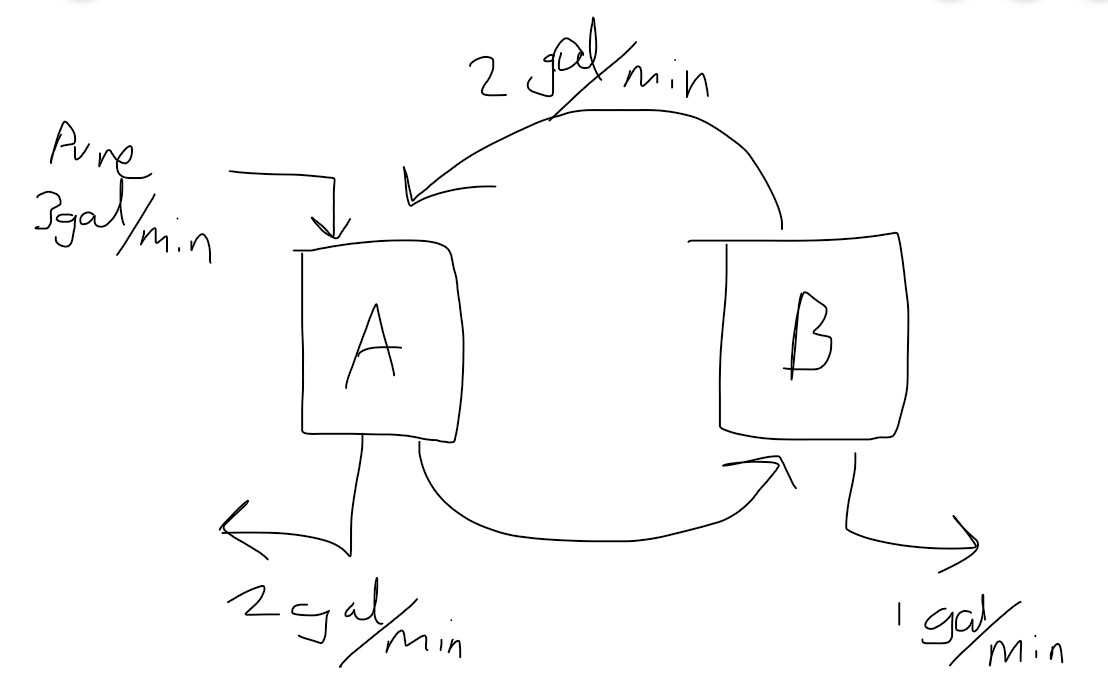
\includegraphics[width=0.8\textwidth]{resource/images/4.4.2 Example 1.jpg}
    \caption{}
    \label{fig:}
  \end{figure}
  Tanks $A$ and $B$ both have 100 gallons of brine. $A$ concentration $0.2 \frac{lb}{gal}$ salt, $B$ concentration is $0.3 \frac{lb}{gal}$. Let $x(t)$ and $y(t)$ be the amounts of salt in tanks $A$ and $B$ in pounds at time $t$(min).
  \begin{align*}
    x'=0+\left( 2 \frac{gal}{min} \right) \left( \frac{y}{100} \frac{lb}{gal} \right)-5 \frac{x}{100} \\
    y'=3 \frac{x}{100}- \frac{3y}{100}\\
    x(0)=20\\
    y(0)=30
  .\end{align*}
  This gives us that \[
    \begin{bmatrix} x\\y \end{bmatrix} '=\begin{bmatrix} -\frac{1}{20}&\frac{1}{50}\\\frac{3}{100}&-\frac{3}{100} \end{bmatrix} \begin{bmatrix} x\\y \end{bmatrix} 
  .\] 
\end{eg}
